\chapter{Luminescent Organic Materials}
\label{chapter: luminscent organic materials}
%%%%%%%%%%%%%%%%%%%%%%%%%%%%%%
\section{Introduction}\label{section: lom introduction}
%%%%%%%%%%%%%%%%%%%%%%%%%%%%%%
Luminescent organic molecules have myriad of useful applications. In aqueous solution they are used extensively in biological imaging, probing, and detection. Deposited as thin films and aggregates, they represent the next generation of organic optoelectronics, where availability and low cost of starting materials, straightforward syntheses, and lightweight devices are attractive features. Perhaps most importantly, the luminescent response of molecular organic systems can be tuned with relative ease compared to their inorganic counterparts, emitting across the visible spectrum and producing white light. 

Since the discovery of electromluminescence in the 1960s, intensive efforts in academia and industry have delivered considerable progress in the field of organic electronics, leading to  the development of applications such as field-effect transistors, photovoltaic cells, optical memory devices, and single-crystal lasers.\cite{Ostroverkhova2016} The most prominent success story is certainly organic light-emitting diodes (OLEDs), which have already reached market adoption for lighting and display purposes. However, in many areas organic systems suffer from low efficiencies, trial-and-error optimisation, and decreased performance in aggregated form versus solution. 

To advance, there must be control over both the supermolecular structure of the material and the electronic structure of the  molecules within.  Unfortunately neither of these properties exist in isolation, and the interplay between them must also be intimately understood, which somewhat complicates matters. Of these three contributing factors, it is the relationship between the electronic structure and the environment which are of interest in this work. The luminescent response of molecules can change drastically from one medium to another, whether in the gas phase, as a solution, aggregated as clusters, or in molecular crystals. Understanding the interplay between the luminophore and its environment is crucial for designing more efficient materials from first principles. 

To this end, we approach this problem using theoretical chemistry methods to investigate organic compounds exhibiting aggregation induced emission (AIE).  AIE-active compounds are non-emissive in dispersed media, but undergo a switch-on of luminescence, typically in the form of fluorescence, upon aggregation. Since organic electronics are manufactured using a solid-state layer, AIE has attracted considerable interest as a pathway to overcome the common effect of aggregation caused quenching (ACQ), hitherto a major obstacle in the development of organic luminophores. In this chapter the problem of ACQ shall be introduced, followed by an examination of the AIE phenomenon through analysis of typical structures, mechanistic interpretations, and how quantum chemical methods are applied to model such systems.
%%%%%%%%%%%%%%%%%%%%%%%%%%%%%%
\section{Aggregation Caused Quenching}\label{section: lom ACQ}
%%%%%%%%%%%%%%%%%%%%%%%%%%%%%%
Photoinduced luminescence occurs after chromophores with $\pi$-conjugation, typically in the form of aromatic moieties, absorb light in the UV/Vis region of the electromagnetic spectrum. In good solvents or dilute concentration, fluorescence will usually follow, although the presence of metals or second row elements can allow phosphorescence via intersystem crossing. Upon aggregation with increased concentration, or crystallisation, the fluorescence is often reduced or quenched completely. 

In 1954, photochemisty pioneer  F\"{o}rster elegantly showed that the fluorescence of pyrene is shifted and weakened with increasing concentration (Figure \ref{figure: Forster_Spectra}).\cite{Forster1954,Forster1969} As the concentration increases, a new fluorescent species is formed and the original band loses intensity. The new band at longer wavelength is a result of the formation of excited dimers, or \textit{excimers}. The presence of aromatic rings in conventional luminophores leads to intermolecular $\pi$-$\pi$ interactions and the formation of dimers. In F\"{o}rster's pyrene example, where the spectra are measured using the same incident wavelength, the single intersecting point shows that the spectrum consists of only two features. The fact that the absorption spectrum is unchanged in the concentration range, the arising band can be ``attributed to an associate that exists only in the excited electronic state, i.e. to an excimer."\cite{Forster1969}
\begin{figure}[H]
\centering
  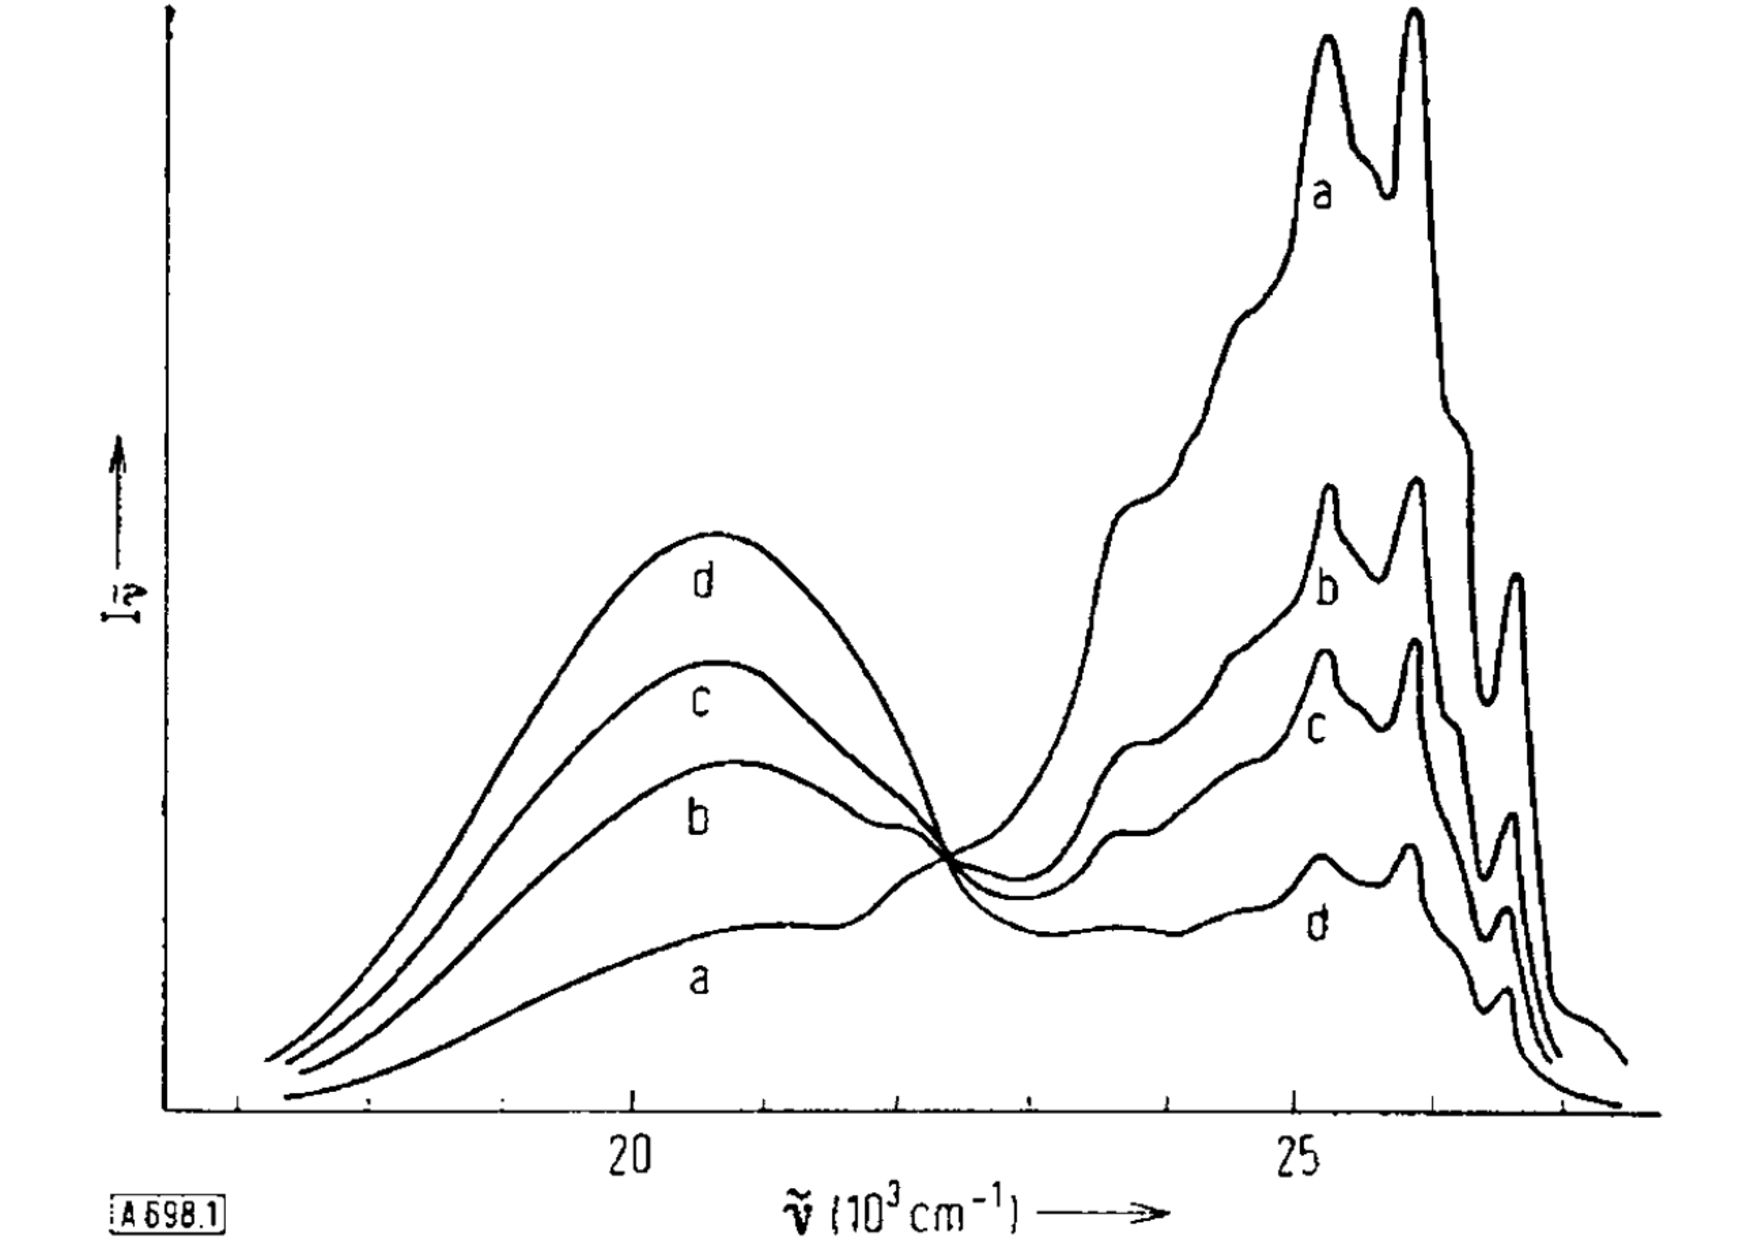
\includegraphics[width=0.6\linewidth]{Intro/Forster_Spectra.pdf}
  \caption[Fluorescence spectrum of pyrene]{Fluorescence spectrum of pyrene (in n-heptane, 20\degree{}C) at different concentrations: a) \SI{5.0e-5}, b) \SI{1.8e-4}, c) \SI{3.1e-4}, d) \SI{7.0e-4}{mol L^{-1}}. Reprinted from ref.~\citenum{Forster1969} with permission of Wiley-VCH.}
  \label{figure: Forster_Spectra}
\end{figure}
The supramolecular alignment of aromatic groups is commonly termed $\pi$-stacking or $\pi$-$\pi$ interactions in the chemical literature. However, this labelling can be slightly misleading and even inaccurate.\cite{Grimme2008,Martinez2012} Grimme argues that a specific $\pi$-$\pi$interaction arises only in large, polyaromatic groups as a result of increased dispersion in specifc orientations.\cite{Grimme2008} Meanwhile, a thorough review of experimental and theoretical literature by Martinez and Iverson found a lack of the face-centred stacking of aromatic groups which would maximise overlap of aromatic $\pi$ clouds.\cite{Martinez2012} They argue that the terms $\pi$-stacking and $\pi$-$\pi$ interactions are misnomers since they incorrectly imply the ubiquity of face-face stacking motifs. Typical stacking motifs are shown in Figure \ref{figure: Benzene_Stacking}, where parallel displacement tempers the unfavourable electrostatic interaction and reduces the Pauli exchange repulsion, with the dominating factor being the favourable dispersion interaction. Inclusion of substituents introduces a permanent dipole, with substituents preferentially aligning antiparallel.\cite{Martinez2012}

\begin{figure}[H]
\centering
  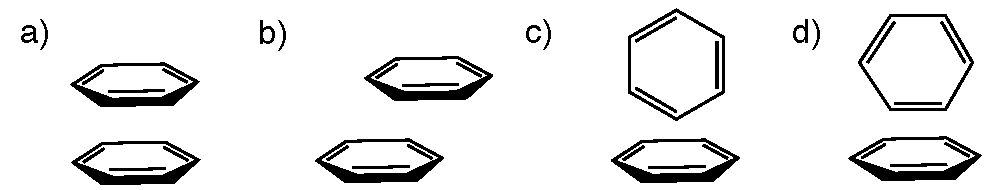
\includegraphics[width=0.7\linewidth]{Intro/Stacking.pdf}
  \caption[Benzene Stacking Motifs]{Packing motifs of benzene molecules: a) face-centred, b) displaced, c) Perpendicular T-shaped, d) Perpendicular Y-shaped. Adapted from ref.~\citenum{Martinez2012}.}
  \label{figure: Benzene_Stacking}
\end{figure}


This intermolecular interaction is detrimental to solid-state fluorescence, and yet is a direct consequence of the design requirements of the chromophore. In biosensing applications, researchers resorted to using dilute solutions with reduced sensitivity because of ACQ.\cite{Thomas2007,Kwok2015} In the solid state, for instance in thin films for optoelectronics, the ACQ effect means that solution screening for viable candidates is rendered meaningless by the differing luminescent properties of the final material compared to the molecule. Strategies to circumvent ACQ have seen varying success, for example through the inclusion of bulky substituents, polar groups, and promotion of hydrogen bonding.\cite{Hong2009,Zhang2013,Mei2014,Mei2015} However, synthetic modification can in turn effect the chromophore's electronic structure and its excited state properties, thus commencing tedious a trail-and-error optimisation process. Attempts to physically block aggregation by encapsulating in surfactants or polymer matrices require extensive engineering and can reduce charge transport.\cite{Hong2009,Chen2000,Lee2013} 

The deleterious effects of ACQ cannot be underestimated and posed a significant problem for organic luminescent applications. Then, in 2001, the group of Ben Zhong Tang found a system which turned the field on its head and opened a new strategy for the design and development of brightly luminescent organic materials. They named the phenomenon aggregation induced emission (AIE). In the next section of this chapter, the roots of AIE shall be examined and the technological advances that have arisen from the discovery.
%%%%%%%%%%%%%%%%%%%%%%%%%%%%%%
\section{Aggregation Induced Emission}\label{section: lom AIE}
%%%%%%%%%%%%%%%%%%%%%%%%%%%%%%
In 2001, the Tang group at the Hong Kong University of Science and Technology were interested in silole-based polymers for highly emissive thin-films. As was common at the time, fabrication of such materials was challenging due to ACQ. Through serendipity during a purification process, they found that a wet spot of 1-methyl-1,2,3,4,5-pentaphenylsilole was almost non-emissive, but brightly fluorescent after solvent evaporation.\cite{Luo2001} The law of aggregation quenching emission had been turned on its head, and the Tang group had observed the exact opposite behaviour, of aggregation inducing light emission. This was almost unheard of for small organic molecules. 

The Tang group used the AIE phenomeon to develop a range of chemical sensors, to detect for instance volatile organic compounds, explosives, and pH.\cite{Dong2007,Li2005,Li2009} Such was the magnitude of the AIE breakthrough and the mechanistic interpretations provided by the Tang group, many other groups began to explore this exciting new phenomenon for a wide range of applications. In the field of biological probing, AIE-active systems can detect important small molecules such as glucose, thiols, and lactic acid.\cite{Wang2014,Yuan2014,Shen2012} Probes have been developed to detect protein fibrillation, which has been linked to Alzheimer's, Parkinson's and type II diabetes.\cite{Hong2012} AIE systems have been also used in medical imaging, where fluorescence is an attractive technique due its high resolution, wide applicability, and low cost.\cite{Mei2015} The Tang group have tracked the progress of the field with periodic, in-depth reviews of the vast number of innovations, of which they contribute a significant share.\cite{Hong2009,Wang2010a,Hong2011,Mei2014,Hu2014,Mei2015}

Upon discovery of AIE, the potential for the improvement of optoelectronic devices was immediately apparent. In the original publication, the group built a highly emissive blue-emitting electroluminescent device, and optimised the device to 8\% external quantum efficiency ($\eta$\textsubscript{QE}) in the cyan region, a vast improvement on the previous high of just 1.5\% for an OLED. \cite{Luo2001,Chen2002} $\eta$\textsubscript{QE} is the product of the electroluminescence (EL) efficiency of the emitter (the organic layer in this case) and the external coupling factor, which is a measure of the fraction of light able to escape the OLED. Due to EL efficiency being limited to 25\% for singlet emitters, and the external coupling being limited to around 22\%, it was previously thought that the theoretical maximum $\eta$\textsubscript{QE} is 5.5\%. Indeed, such was the remarkable $\eta$\textsubscript{QE} measure in this OLED that these previously accepted limitations had to be reconsidered.

In follow-up work, a light-blue emitting OLED with hexaphenylsilole (Figure \ref{figure: HPS_TPE}) as the emitting layer was fabricated with $\eta$\textsubscript{QE} of 7\%.\cite{Chen2003} While the unfavourable spin statistics inhibit efficiency for singlet-emitting OLEDs across the visible spectrum, deep blue emitters are harder still since the large band gap makes charge injection difficult, hindering the development of full colour displays. Non-doped deep blue OLEDs with $\eta$\textsubscript{QE} of around 4\% were reached in 2014, with emitters based on triphenylamine and tetraphenylethene (Figure \ref{figure: HPS_TPE}).\cite{Huang2014,Huang2014a} This has recently been increased to 6.5\% using a carbazole-based organic layer, and in 2018 reached 9.4\%.\cite{KumarKonidena2017,Tang2018} This represents a high for non-doped singlet blue emitters. Inclusion of phosphorescent or thermally-activated delayed fluorescent dopants can further increase the quantum efficiency by harvesting triplet states for luminescence.\cite{Zhu2018}

\begin{figure}[H]
\centering
  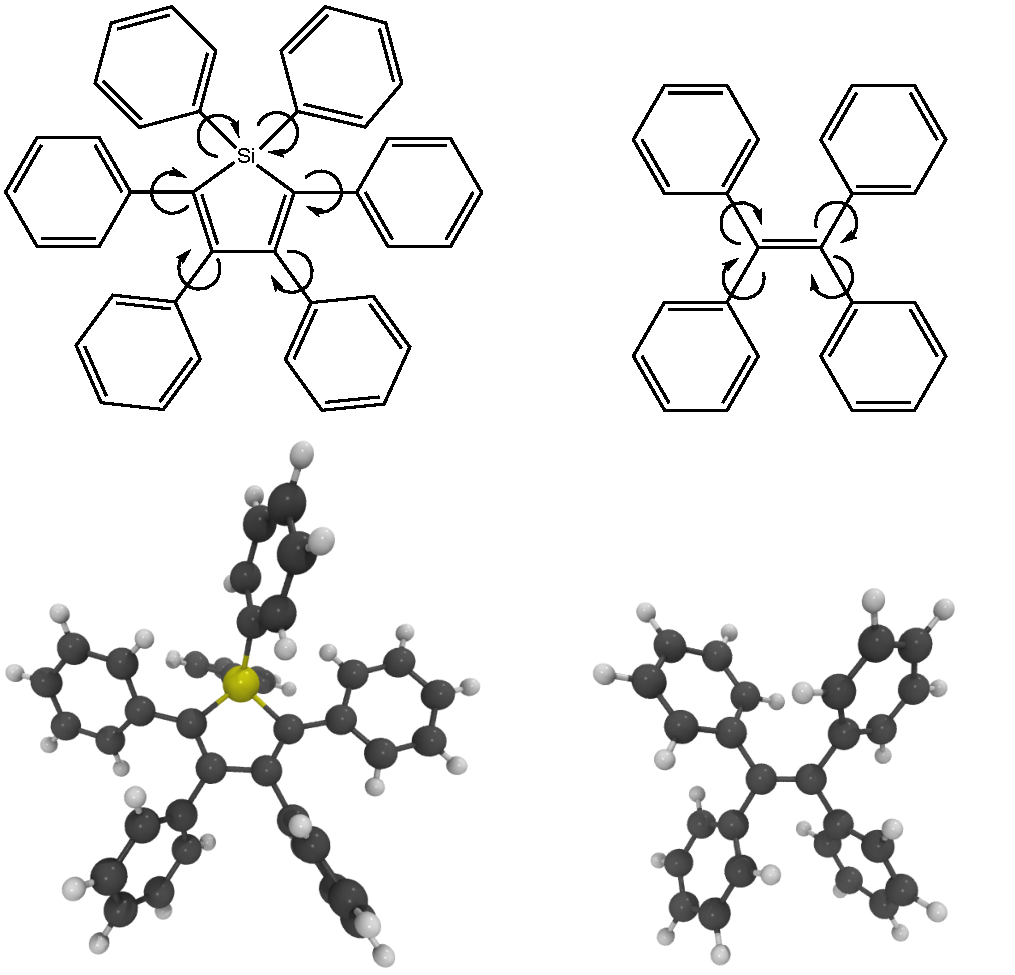
\includegraphics[width=0.7\linewidth]{Intro/HPS_TPE.pdf}
  \caption[Examples of AIE-active chromophores]{Two dimensional (top) and three dimensional (bottom) structures of two of the ubiquitous AIE-active systems, hexaphenylsilole (HPS, left) and tetraphenylethene (TPE, right). AIE occurs through restriction of the rotational motions depicted with arrows.}
  \label{figure: HPS_TPE}
\end{figure}

Systems exhibiting AIE are typically based on a propeller architecture, where a central stator is connected to a number of aromatic rotors via single bonds, as shown in Figure \ref{figure: HPS_TPE}. In the initial analysis of 1-methyl-1,2,3,4,5-pentaphenylsilole, the absorption spectra showed that after the water fraction in an ethanol-water solvent mixture rose above 60\%, the absorption band increased in intensity and moved to longer wavelengths.\cite{Luo2001} On this basis, the AIE activity was attributed to the formation of aggregates which forced the molecules into a more planar conformation, thus increasing the conjugation and the absorption. Enough rotation about the sigma bonds was still possible to prevent complete planarity and therefore limiting the stacking and subsequent fluorescence quenching. 

A few months later, the group showed the AIE effect for four more silole systems, followed by an extensive study of ten phenylsiloles.\cite{Tang2001,Chen2003} Crucially, in this later work the crystal structure of the siloles showed that the conformation remains twisted in the solid state.\cite{Chen2003} Large torsional angles exist between the phenyl groups and the central silole moiety, on account of the steric repulsion between the six phenyl groups. The lack of space between the phenyl blades, and their angular orientations, prevents intermolecular stacking which give rise to aggregation caused quenching. Therefore the planarisation hypothesis was wrong. 

Twisted intramolecular charge transfer (TICT) was a known inhibitor of fluorescence, where a non-emissive twisted conformer is formed via charge separation in the chromophore. The TICT state can be stabilised, and thus favoured, in polar solvents. However, no emission was recorded across a wide range of solvent polarities for the siloles, ruling out TICT as the cause for AIE. Also, the lack of electron donor and acceptor groups make it highly unlikely that TICT could take place in the siloles. In an elegant experiment it was found that the emission increased almost linearly with increasing solvent viscosity, even though no aggregates were formed. In a similar vain, the photoluminescence intensity increased with decreasing temperature, with NMR studies confirming that the intramolecular rotations of the exterior phenyl groups were reduced at lower temperatures. It was concluded the in good solvents, at ambient temperature, the energy consumed by the rotation of the phenyl groups about the single bonds results in the nonradiative decay of the excited state decay. Upon aggregation, the propeller-like shape limits the intermolecular stacking. Strong C-H\textperiodcentered\textperiodcentered\textperiodcentered$\pi$ interactions rigidify the structure, hindering the intramolecular rotation and the excited state decays via fluorescence.\cite{Chen2003}

The restriction of intramolecular rotation (RIR) mechanism allowed the library of AIE-active systems to be expanded to other molecules with propeller-shaped structures propeller.  Along with the phenylsiloles, tetraphenylethene (TPE)  derivatives have driven understanding and technological progress in the field.\cite{Hong2009,Wang2010a,Hong2011,Mei2014,Hu2014,Mei2015} By switching a phenyl group of TPE with a traditional ACQ molecules, such as triphenylamine or carbazole, the electroluminscence properties of the system are enhanced due to the hole-transport properties of the ACQ group.\cite{Chan2014} Conversely, ACQ cores can be made to undergo AIE by the attachment of TPE.\cite{Yuan2010a}

Dissipation of the excited state can occur through means other than rotation. A bent, $\pi$-surface system of benzenes fused with cyclooctatetraenes undergoes AIE but without any rotable units.\cite{Nishiuchi2013} In solution, ring inversions dissipate the excited state and there is almost no emission. Single crystals show emission in the blue region, since the bent structure prevents facial stacking and the inversion modes are restricted. Thus AIE is achieved through restriction of intramolecular vibrations (RIV). In a similar vain, the RIV mechanism can be applied to TPE by locking pairs of phenyl groups with eythlene linkers. In 2014, Tang unified the RIR and RIV interpretations under the restriction of intramolecular motions (RIM) umbrella.\cite{Leung2014}

The discovery and development of the AIE phenomenon has transformed the field of luminescent organic materials. While much of the innovation has been based on the propeller systems, a class of systems based on excited state intramolecular proton transfer (ESIPT) have attracted interest in recent years for their favourable photochemical properties. ESIPT systems form the basis of the research in this thesis. In the next section the ESIPT mechanism shall be introduced, along with the key applications which incorporate ESIPT-active systems.
%%%%%%%%%%%%%%%%%%%%%%%%%%%%%%
\section{Excited State Intramolecular Proton Transfer}\label{section: lom ESIPT}
%%%%%%%%%%%%%%%%%%%%%%%%%%%%%%
Tautomerism is a type of isomerism resulting in the transfer of a chemical group (usually a proton) between two sites on a molecule, and simultaneous switching of a single and double bond. Photo-induced tautomerism, where the transferring group is a proton, is called excited state intramolecular proton transfer (ESIPT). Research into the mechanism and potential applications has been active for more than half a century, since ESIPT was first observed in the 1950s in salycylic acid. Photochromic materials harnessing ESIPT have garnered much attention due to the wide range of applications and remarkable properties. In particular, it is the unusually large Stokes-shifted emission which makes ESIPT so attractive. The separation between the absorption and emission wavelengths can typically exceed 200 nm, reducing self-absorption and increasing the output signal for the desired application. The emission colour can be tuned by the addition of electron donating or withdrawing groups, as well as solvent polarity and viscosity.\cite{Azarias2016,Yushchenko2007} Dual emission from the pre- and post-ESIPT forms is also possible. These characteristics, in tandem with AIE, have resulted in ESIPT chromophores being used for chemical sensing, biological imaging and probing, as well the optoelectronic applications such as optical memory, lasers, and OLEDs.\cite{Hsieh2010,Kwon2011,Zhao2012,Demchenko2013,Padalkar2015,Chen2018}
\begin{figure}[H]
\centering
  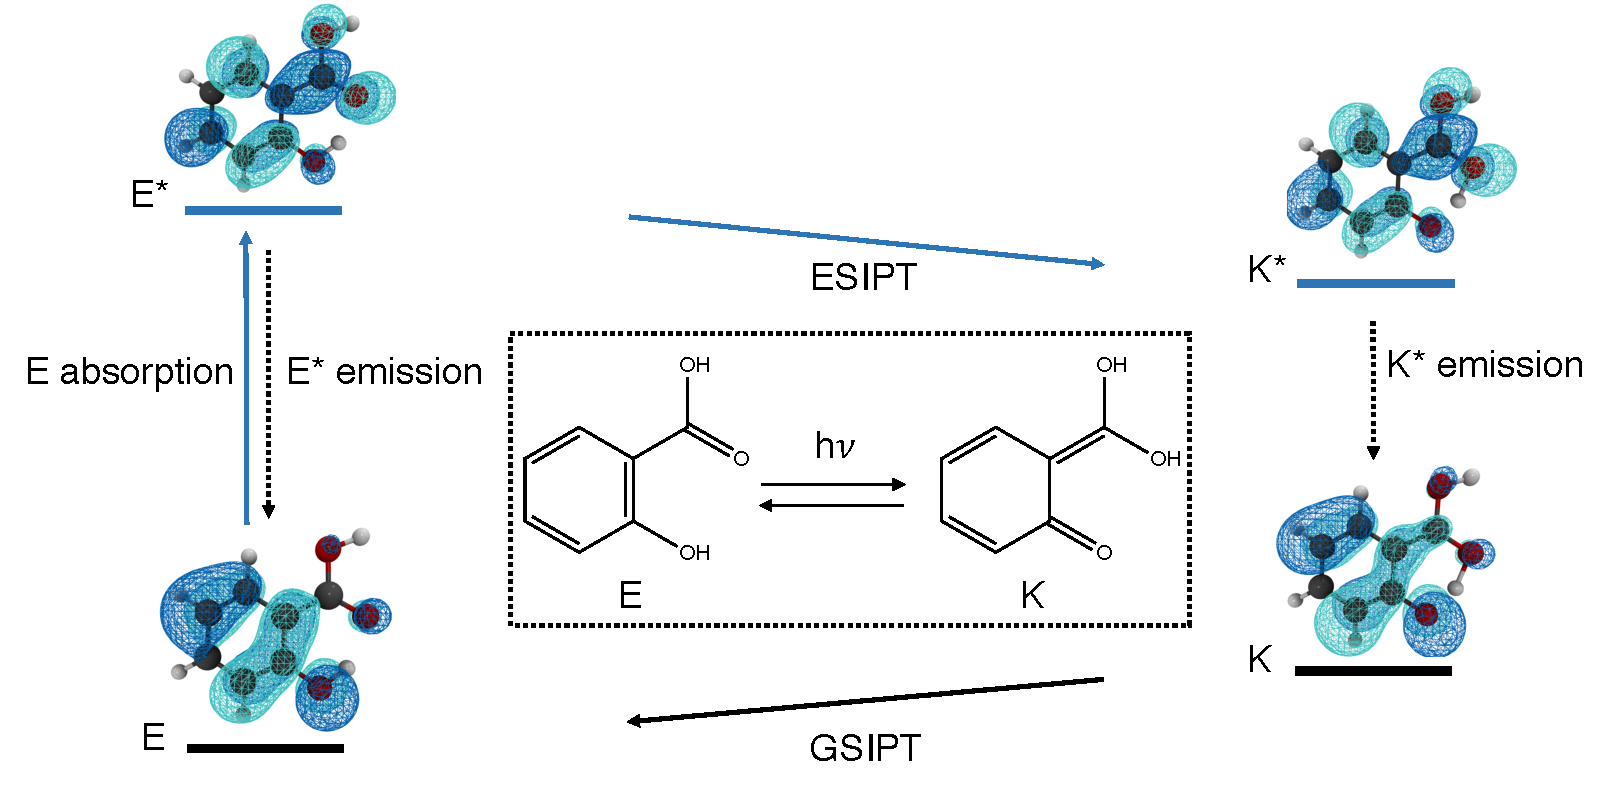
\includegraphics[width=0.95\linewidth]{Intro/ESIPT.pdf}
  \caption[The four-level photocycle of ESIPT]{The four-level photocycle of ESIPT for salyclic acid. The HOMO and LUMO orbitals for tautomer are also shown to represent the change of electronic density distribution.}
  \label{figure: ESIPT}
\end{figure}
Inherent in all ESIPT processes is a fully reversible four-level photocycle, the prerequisite for which is the presence of an intramolecular hydrogen bond. The proton donor can be an amino or hydroxyl group, while the proton acceptor is usually an imine or carbonyl. The four-level photocycle for salycylic acid is depicted in Figure \ref{figure: ESIPT}, along with the main molecular orbitals. The chromophore in the ground state (S\textsubscript{0}) is in the enol form (E), mediating hydrogen bond formation between the carbonyl oxygen and the hydroxyl proton. Upon electronic excitation, the excited state (E$^\ast$, S\textsubscript{0}) the geometry remains unchanged but electronic redistribution acidifies the hydroxyl and increases the basicity of the carbonyl group, as a result of the population of the $\pi^\ast$ orbital on the carbonyl oxygen. In the excited state, the keto form (K$^\ast$) is more stable due to the redistributed electron density, and the proton migrates from the hydroxyl oxygen to the carbonyl oxygen. Depending on the system, fluorescence can occur from both the excited enol form (E$^\ast$) and the excited keto form (K$^\ast$), although due to the ultrafast nature of the proton transfer the major emitting species is the keto tautomer.\cite{Zhao2012} For most ESIPT processes containing strong hydrogen bonds, proton transfer is near barrierless and  occurs on a femtosecond time scale.\cite{Padalkar2015} The rate of the proton transfer and emission wavelength are highly sensitive to the surrounding medium and the presence of electron donor/acceptor moieties.\cite{Demchenko2013,Lin2017a,Li2017c} After fluorescence, the ground state keto form (K) is populated and the four level photocycle (E$\rightarrow$E$^{\ast}$$\rightarrow$K$^{\ast}$$\rightarrow$K) is completed. Ground state intramolecular proton transfer (GSIPT) will restore the intial geometry, although other photoproducts can be formed, for instance through cis-trans isomerisation or intersystem crossing.\cite{Al-Soufi1990}

AIE in ESIPT chromophores can be more complex that in the non-polar propeller systems discussed earlier. The presence of hydrogen bonding sites enables the formation of intermolecular hydrogen bonds with solvent molecules, weakening the intramolecular bond and hindering ESIPT.\cite{Cheng2015f} Kasha showed that the ratio of fluorescence intensity between E$^\ast$ and K$^\ast$ dramatically changes based upon the solvent polarity.\cite{Kasha1986} In 3-hydroxyflavanone, the K$^\ast$ fluorescence band is suppressed and the E$^\ast$ band increases in intensity with polar solvents. In strongly basic solvents, intermolecular proton transfer can occur between the chromophore and solvent, blocking access to the K$^\ast$ state\cite{Laurent2014}. As touched upon earlier, the presence of donor acceptor groups opens the possibility of deactivation through twisted intramolecular charge transfer (TICT). In solvent, the TICT state is populated after proton transfer and lead to nonradiative decay. In a similar vain to RIR, aggregation frustrates the torsional mode, preventing the TICT from forming, and opens the radiative decay channel.\cite{Park2017,Wu2015a}

The most investigated class of ESIPT molecules are based on benzothiazole dyes, particularly 2-(2-hydroxyphenyl)benzothiazole (HBT).\cite{Padalkar2015,Kwon2011} The groups of Li and Liu investigated the effect of solvent for a range of HBT derivatives, finding that increasing polarity impedes the proton transfer reaction and diminishes fluorescence. This is compounded by highly polar, protic solvents, where the hydroxyl proton can dissociate to form the phenolic anion. The proton transfer is highly sensitive to the solvent polarity, which is highly useful for sensing and probing applications.\cite{Wang2009,Cheng2015f} A HBT analogue has been developed for ratiometric probing for hydrogen peroxide in living cells, where the ESIPT-active fluorophore is produced by oxidative hydrolysis.\cite{Tang2018a} HBT-based systems are also applicable for pH sensing, ion detection, biothol probing, and intracellular imaging.\cite{Kachwal2018,Kachwal2018,Liu2018}

Substitution of electron donor and acceptor groups onto ESIPT cores can alter the proton transfer rate and stability of the enol and keto conformers on the excited state potential energy surface. In an extensive theoretical study, Jacquemin and co-workers investigated how different substitution patterns affect the emission from enol and keto states for a range of ESIPT systems based on HBT, hydrophenyl-benzoxazole (HBO) and hydroxyphenyl-indole (HI).\cite{Azarias2016} They found that dual emission from both E$^*$ and K$^*$ is only possible in a small energy window for the compounds tested, and that the K$^*$ minimum can be favoured more drastically by changing the core from HBO to HI rather than by any sole substituent effect. The strongest substituent effects are seen with electron donor groups, such as methoxy, which stabilise the E$^*$ state. The K$^*$ state can be favoured by electron withdrawing groups in particular positions. Crucially, the effects of combining substituent groups is complex and depend on the specific ESIPT-core and substituent combination. The easily purturbed electronic structure of these systems make design from first principles extremely challenging.

ESIPT cores are excellent candidates for optoelectronicelectronic applications on account of minimised self-absorption. However, the environment sensitivity which makes them so suitable for probing can be harmful to device stability.\cite{Kwon2011} Through chemical modifacations, the Park group have fabricated stable OLED devices with a range of emission frequencies, with carbazole .\cite{Park2008,Park2009,Kim2011} Introduction of carbazole gave access to blue K$^*$ emission.\cite{Park2008} $\eta$\textsubscript{QE} values of 14\% have been reached by incorporating triplet harvesting via thermally activated delayed fluorescence with ESIPT.\cite{Mamada2017} Emission from both E$^*$ and K$^*$ enables white-light emission in devices, a highly attractive property due to the rarity of single molecule fluorophores with wide emission bands.\cite{Tang2011,Yao2011,Zhang2016b,Serdiuk2017}






